\documentclass[]{exam}
\usepackage{epic,array,ecltree,url,calrsfs}
\usepackage[nointegrals]{wasysym}

%These tell TeX which packages to use.
\usepackage{array,epsfig}
\usepackage{amsmath}
\usepackage{amsfonts}
\usepackage{amssymb}
\usepackage{amsxtra}
\usepackage{amsthm}
\usepackage{mlextra} % must come after ams packages
\usepackage{mathrsfs}
\usepackage[dvipsnames]{xcolor}
\usepackage{array}
\usepackage{graphicx}
\graphicspath{ {../art/} }
\usepackage{bm}
\usepackage{tikz}
\usepackage{multicol}
\usepackage{enumitem}

\newcommand{\twonode}{%
  \begingroup\normalfont
  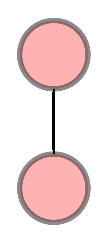
\includegraphics[height=\fontcharht\font`\b]{2nodetree.eps}%
  \endgroup
}


\title{Lab 3: The Weak, the Strong and the Mutual}
\author{Foundations of Computer Science}
\date{\today}
%\pagestyle{empty} 
%\footer{}{\thepage}{}

\printanswers
\unframedsolutions
\SolutionEmphasis{\itshape\small}
\SolutionEmphasis{\color{NavyBlue}}


\begin{document}

\maketitle

\setlength{\columnseprule}{1pt}
\begin{questions}


\question Consider the following recursive definitions of sets of strings
(left) and the three induction rules listed (right).  For each of the 
claims made about these sets below, choose the induction rule most suitable 
for proving the claim. 
\begin{multicols}{2}
{\bf Recursive Definitions:}\\
\begin{enumerate}
\item
\begin{tabbing}
{\bf R2}XX \=  \kill
{\bf B1} \>
        \(\begin{array}[t]{l}
        aa \in S_1
        \end{array}\) \\[2ex]
{\bf B2} \>
        \(\begin{array}[t]{l}
        \epsilon \in S_1
        \end{array}\) \\[2ex]
{\bf R} \>
        \(\begin{array}[t]{l}
        x \in S_1 \;\;\;y \in S_1 \\
        \hline
        xy \in S_1
        \end{array}\)
\end{tabbing}
\hrule
\item
\begin{tabbing}
{\bf R2}XX \=  \kill
{\bf B} \>
        \(\begin{array}[t]{l}
        a \in S_2
        \end{array}\) \\[2ex]
{\bf R} \>
        \(\begin{array}[t]{l}
        x \in S_2 \;\;\;y \in S_2 \\
        \hline
        xyx \in S_2
        \end{array}\)
\end{tabbing}
\hrule

\item
\begin{tabbing}
{\bf R2}XX \=  \kill
{\bf B} \>
        \(\begin{array}[t]{l}
        a \in S_3
        \end{array}\) \\[2ex]
{\bf R} \>
        \(\begin{array}[t]{l}
        x \in S_3 \\
        \hline
        xbx \in S_3
        \end{array}\)
\end{tabbing}
\end{enumerate}

\columnbreak
{\bf Induction Rules:}\\
\begin{tabbing}
[1]XX \=  \kill
[1] \>
	\(\begin{array}[t]{l}
	S(i) \;\wedge\; \forall n \geq i.\;S(n) \Rightarrow S(n+1) \\
	\hline
	\forall n \geq i. \; S(n)
	\end{array}\) % \\[2ex]
\end{tabbing}

\begin{tabbing}
[2]XX \=  \kill
[2] \>
	\(\begin{array}[t]{l}
	S(i) \;\wedge\; \forall n \geq i.\;S(i)\;\wedge\;S(i+1)\;\wedge\cdots\wedge\;S(n) \Rightarrow S(n+1) \\
	\hline
	\forall n \geq i. \; S(n)
	\end{array}\)
\end{tabbing}

\begin{tabbing}
[3]XX \=  \kill
[3] \>
	\(\begin{array}[t]{l}
	S(i) \;\wedge\; S(i+1)\;\wedge\cdots\wedge\;S(j)\;\wedge\; \\
\forall n \geq j.\;S(i)\;\wedge\;S(i+1)\;\wedge\cdots\wedge\;S(n) \Rightarrow S(n+1) \\
	\hline
	\forall n \geq i. \; S(n)
	\end{array}\) % \\[2ex]
\end{tabbing}
~\\
~\\
~\\
~\\
    
\end{multicols}
\textbf{Claims:}
\begin{solution}
Note that there can be more than one possible proof for a given claim, so
there are multiple acceptable answers, though some are more obvious than
others. In the solutions below, the choice corresponding to what seems
like the most obvious approach is given, along with a brief description
of that approach.
\end{solution}
\begin{parts}
\part All elements of $S_1$ have even length.
\begin{solution}
Rule [2]. Strong induction over derivation height using a single base case.
\end{solution}

\part All elements of $S_2$ have odd length.
\begin{solution}
Rule [2]. Strong induction over derivation height using a single base case.
\end{solution}

\part All elements of $S_3$ begin and end in $a$. 
\begin{solution}
Rule [1]. Weak induction over derivation height using a single base case.
\end{solution}

\part All odd length strings of $a$'s are contained in $S_2$.
\begin{solution}
Rule [1]. Weak induction over the natural numbers, where $k \in \N$ and the $k^{th}$ 
odd length string of $a$'s is defined as the unique string of $a$'s with length $2k-1$. 

Note that it would also be possible to use Rule [3] and perform strong induction 
over strings of length $k$ where
$S(k)$ is written as ``If $x$ is a string of $a$'s with length $k$ and $k$ is
odd, then $x \in S_2$.'' In this approach, you would likely need two base cases:
one in which $k$ is odd and one in which $k$ is even. Although the structure
of this argument is more complicated, it avoids the need
to give a special definition of the set of odd length strings of $a$'s.
\end{solution}

\end{parts}
\question What is the meaning of $j$ in the third induction rule? What does it
represent, and what determines its value relative to $i$?
\begin{solution}
$j$ represents the index of the last base case. If there are
$b$ base cases, the value of $j$ will be $i + b - 1$.
\end{solution}

\question Referencing the definition of rooted trees given in the slides,
draw the structure produced in the following derivation:
\begin{center}
\begin{tabular}{lllll}
  $\bid{B}$  & $\id{nil}\in\id{RTL}$            &                       & &
  \\ \cline{2-2} 
  $\bid{R2}$ & $\id{node}(\id{nil})\in\id{RT}$  & $\id{nil}\in\id{RTL}$ & $\bid{B}$ &
  \\ \cline{2-3}
  $\bid{R1}$ & \multicolumn{2}{l}{ $\id{cons}(\id{node}(\id{nil}),\id{nil})\in\id{RTL}$} & & 
  \\ \cline{2-3}
  $\bid{R2}$ & \multicolumn{2}{l}{ $\id{node}(\id{cons}(\id{node}(\id{nil}),\id{nil}))\in\id{RT}$} & $\id{nil} \in \id{RTL}$ & $\bid{B}$
  \\ \cline{2-4}
  $\bid{R1}$ &
  \multicolumn{3}{l}{$\id{cons}(\id{node}(\id{cons}(\id{node}(\id{nil}),\id{nil})), \id{nil})\in\id{RTL}$}
\end{tabular}
\end{center}
\vspace{-5mm}
\begin{solution}
$[\twonode]$
\end{solution}

\question What is the derivation height of the following tree:  

\begin{center}
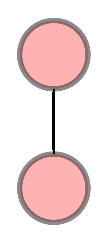
\includegraphics[height=2cm]{2nodetree.eps}%
\end{center}
\vspace{-5mm}
\begin{solution}
3
\end{solution}

\question Reproduced below is the argument from slide $6$ of the mutual
induction slide set, which proves that the number of edges in a rooted
tree list, $l'$, of derivation height $n + 1$ is equal to the number of nodes
in the list, minus the length of the list. Work through each of the
steps below and annotate each line by adding a plain-language explanation as to 
why it follows from the line above. (Feel free to reference the original slides
as needed).

\begin{displaymath}
\begin{array}{llll}
1. & \id{\#edges}(l') & = &\id{\#edges}(\id{cons}(t,l)) \\
2. &  & = & \id{\#edges}(t) + \id{\#edges}(l) \\
3. & 	& = & \id{\#nodes}(t) - 1 + \id{\#edges}(l) \\
4. & 	& = & \id{\#nodes}(t) - 1 + \id{\#nodes}(l) - |l| \\
5. & 	& = & \id{\#nodes}(\id{cons}(t,l)) - 1 - |l| \\
6. & 	& = & \id{\#nodes}(\id{cons}(t,l)) - (1 + |l|) \\
7. & 	& = & \id{\#nodes}(\id{cons}(t,l)) - |\id{cons}(t,l)|\\
8. & 	& = & \id{\#nodes}(l') - |l'|
\end{array}
\end{displaymath}
\begin{solution}
omitted
\end{solution}

% MAYBE NEXT WEEK
%
%Recall that a ``leaf'' node is a node with no children
%and an ``internal'' node is a node with children.
%
%Recall that a full binary tree is one in which each internal
%node has exactly two children.
%
%Write a Post System for full binary trees.
%
%Let L be the number of ``leaf'' nodes and I be the number of internal nodes.
%Prove that, for all full binary trees, L = I + 1.



\end{questions}
\end{document}


